\documentclass[9pt,aspectratio=169]{beamer}

% --- Theme ---
\usetheme{Singapore}
\setbeamertemplate{navigation symbols}{}   % no icons
\setbeamertemplate{mini frames}{}          % no dots in headline
\setbeamercovered{transparent}

% --- Grayscale colors ---
\definecolor{PelloGrayDark}{RGB}{60,60,60}
\definecolor{PelloGray}{RGB}{120,120,120}
\definecolor{PelloGrayLight}{RGB}{235,235,235}
\definecolor{PelloGrayUltraLight}{RGB}{248,248,248}

\usecolortheme[named=PelloGrayDark]{structure}

% --- Blocks ---
\setbeamertemplate{blocks}[rounded][shadow=false]
\setbeamercolor{block title}{fg=white,bg=PelloGrayDark}
\setbeamercolor{block body}{fg=black,bg=PelloGrayLight}
\setbeamercolor{block title example}{fg=white,bg=PelloGrayDark}
\setbeamercolor{block body example}{fg=black,bg=PelloGrayLight}
\setbeamercolor{section in head/foot}{fg=PelloGray,bg=PelloGrayLight}
\setbeamercolor{subsection in head/foot}{fg=PelloGray,bg=PelloGrayLight}
\setbeamercolor{frametitle}{fg=black}

% --- Itemize bullets (optional; keep if you like the style) ---
\setbeamertemplate{itemize item}{\raisebox{0.2em}{\scalebox{.6}{$\bullet$}}}
\setbeamertemplate{itemize subitem}{\raisebox{0.2em}{\scalebox{1}{$-$}}}

% --- Footer: frame numbers ---
\makeatletter
\setbeamertemplate{footline}{%
  \hfill\usebeamerfont{footline}\insertframenumber/\inserttotalframenumber\hspace{1em}\vspace{2pt}
}
\makeatother

% --- Minimal packages (add more only when needed) ---
\usepackage[english]{babel}
\usepackage[T1]{fontenc}
\usepackage[utf8]{inputenc}
\usepackage{graphicx}
\usepackage{tikz}
\usepackage{booktabs}
\usepackage{makecell} % for jumping lines within cells in tables.
\usepackage{multirow}
\usepackage{amsmath,amssymb,bm}
\usepackage{hyperref}
\hypersetup{colorlinks,linkcolor=,urlcolor=blue}
\usepackage{comment}
\usepackage{listings}
\lstset{
  language=R,
  basicstyle=\ttfamily\footnotesize,
  keywordstyle=\color{blue},
  commentstyle=\color{green!50!black},
  stringstyle=\color{red},
  frame=single,
  showstringspaces=false
}
\linespread{1.7}   % 1.0 = normal, 1.2–1.5 common
\AtBeginEnvironment{lstlisting}{\linespread{1}\selectfont} % keep code listings single-spaced



% --- Macros ---
\newcommand{\E}{\mathbb{E}}
\newcommand{\Var}{\mathrm{Var}}
\newcommand{\Cov}{\mathrm{Cov}}
\newcommand{\plim}{\operatorname{plim}}
\newcommand{\SEhat}{\widehat{SE}}
\newcommand{\indep}{\perp\!\!\!\perp}
\usetikzlibrary{arrows.meta,positioning}
\tikzset{ % causal diagrams
  -Latex, auto, node distance=1cm and 1.2cm, semithick,
  state/.style={circle, draw=PelloGrayDark, fill=PelloGrayLight, minimum size=8mm, inner sep=0pt},
  bidirected/.style={Latex-Latex, dashed},
  control/.style={rectangle, rounded corners, draw=PelloGrayDark, fill=PelloGrayLight, minimum height=8mm, inner sep=3pt}
}

% --- Meta ---
\title{Applied Economics}
\subtitle{Multiple Linear Regression, Causality, and Inference}
\author{Pello Aspuru}
%\institute{University of Vienna}
\date{Winter 2026/2027}

% --- Title page spacing + bottom-left author/date ---
\setbeamertemplate{title page}{
  \vspace{8em}
  \begin{center}
	{\usebeamerfont{title}\inserttitle\par}
  	\vspace{1.5em} % <-- increase title–subtitle gap
  {\usebeamerfont{subtitle}\insertsubtitle\par}
  \end{center}
  \vspace{4em}
  \begin{flushleft}
    {\usebeamerfont{author}\insertauthor\par}
    {\usebeamerfont{date}\insertdate}
  \end{flushleft}
}

\begin{document}

% Title slide without headline/footer
{
  \setbeamertemplate{headline}{}
  \setbeamertemplate{footline}{}
  \begin{frame}
    \titlepage
  \end{frame}
}

\begin{frame}{Plan for this Lecture}
\linespread{1.2}\selectfont
  \begin{enumerate}
    \item The causal question: potential outcomes, ATE, ATT
    \item Regression as a tool: what $\hat\beta$ measures and when it is causal
    \item Why OLS fails: one formula, three sources of endogeneity
    \item Inference: robust and clustered standard errors
    \item Bridge: what IV, panel FE, DiD and RDD each assume instead of $\E[u_i\mid X_i]=0$
  \end{enumerate}
\end{frame}

\section{The Causal Question}

\begin{frame}{The Multiple Linear Regression Model}
\linespread{1.2}\selectfont
  \[
    Y_i = \beta_0 + \beta_1 X_{1i} + \beta_2 X_{2i} + \dots + \beta_k X_{ki} + u_i, \qquad i=1,\dots,N
  \]
  \vspace{-0.2cm}
  \begin{columns}[c]
  \begin{column}{0.58\textwidth}
  \begin{itemize}
    \item $i$: unit of observation in the population.
    \item $Y_i$: \textbf{dependent variable} (outcome).
    \item $X_{1i}$: \textbf{treatment} variable, our main focus.
    \item $\beta_{1}$: coefficient for the treatment, \textbf{same} for all $i$. \pause
    \item $X_{2i},\dots,X_{ki}$: \textbf{covariates} (controls), observed.
    \item $\beta_{ki}$: coefficient for the $k$-th control variable.
    \item $u_i$: \textbf{error term}: all \emph{unobserved} determinants of $Y_i$.
  \end{itemize}
  \end{column}
  \begin{column}{0.40\textwidth}
  \centering
  \onslide<1->{
  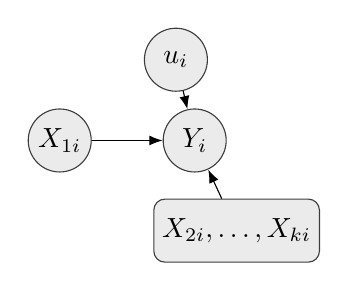
\begin{tikzpicture}[node distance=0.45cm and 0.9cm]
    \node[state] (x) at (0,0) {$X_{1i}$};
    \node[state] (y) [right =of x] {$Y_i$};
    \node[state] (u) [above right =of x] {$u_i$};
    \node[control] (c) [below right =of x] {$X_{2i},\dots,X_{ki}$};
    \path (x) edge (y);
    \path (u) edge (y);
    \path (c) edge (y);
    %\path[bidirected] (x) edge[bend right=10] (c);
  \end{tikzpicture}}
  \end{column}
  \end{columns}
  \medskip
  \pause
  \begin{block}{}
    \begin{itemize}
      \item Correlation: a statistical \textbf{measure} describing the relation between treatment $X_{1i}$ and outcome $Y_i$.
      \item Causality: a \textbf{claim} about the effect of $X_{1i}$ on $Y_i$, holding the controls and $u_i$ fixed.
      %\item[$\rightarrow$] Correlations \textbf{may} support causal claims.
    \end{itemize}
  \end{block}
\end{frame}

\begin{frame}{Potential Outcomes}
  $
    Y_i = \beta_0 + \beta_1 X_{1i} + \beta_2 X_{2i} + \dots + \beta_k X_{ki} + u_i, 
    \qquad i=1,\dots,N
    \qquad X_{1i} \in \{0,1\}
  $
  \begin{itemize}
    \item $Y_i(0) = \beta_0 + \beta_1 \cdot 0 + \beta_2 X_{2i} + \dots + \beta_k X_{ki} + u_i$: outcome of $i$ without treatment.
    \item $Y_i(1) = \beta_0 + \beta_1 \cdot 1 + \beta_2 X_{2i} + \dots + \beta_k X_{ki} + u_i$: outcome of $i$ with treatment.
  \end{itemize}
  \pause
  \vspace{0.3cm}
  Each unit belongs to either the treated or control group and has two \textbf{potential outcomes}:
  \begin{center}
    \begin{tabular}{@{}lcc@{}}
      \toprule
      & $X_{1i}=1$ (treated) & $X_{1i}=0$ (control) \\
      \midrule
      %Potential outcomes & $Y_i(1)$, $Y_i(0)$ & $Y_i(1)$, $Y_i(0)$ \\
      Observed outcome  & $Y_i=Y_i(1)$ & $Y_i=Y_i(0)$ \\
      Missing (counterfactual) & $Y_i(0)$ & $Y_i(1)$ \\
      \bottomrule
    \end{tabular}
  \end{center}
  \vspace{0.3cm}
  Causal effect of $X_{1i}$ on \textbf{individual} unit $i$: \quad $Y_i(1) - Y_i(0)$
   $\quad \rightarrow \quad$
    Cannot be computed.
\end{frame}

\begin{frame}{From Individual Effects to Group Comparisons}
\linespread{1.2}\selectfont
   Average Treatment Effect (ATE): compares the mean outcomes between the two groups:
  \[
    ATE = 
    \underbrace{\E[Y_i(1)\mid X_{1i}=1]}_{\text{Treated}} - \underbrace{\E[Y_i(0)\mid X_{1i}=0]}_{\text{Control}}
  \]
  Adding and subtracting the treated group's missing counterfactual...
  \begin{align*}
    ATE&= \E[Y_i(1)\mid X_{1i}=1] \textcolor{red}{{}- \E[Y_i(0)\mid X_{1i}=1] + \E[Y_i(0)\mid X_{1i}=1]{}} - \E[Y_i(0)\mid X_{1i}=0]\\
    &= {\underbrace{\E[Y_i(1)-Y_i(0)\mid X_{1i}=1]}_{\text{causal effect (on the treated)}}} +\underbrace{\E[Y_i(0)\mid X_{1i}=1]-\E[Y_i(0)\mid X_{1i}=0]}_{\text{selection bias}}
  \end{align*}
  Comparing units with the same observed controls, $\boldsymbol{X}_i = (X_{2i},\dots,X_{ki})$:
  \[
    ATE = \underbrace{\E[Y_i(1)-Y_i(0)\mid X_{1i}=1, \boldsymbol{X}_i]}_{\text{causal effect (on the treated)}} + \underbrace{\E[Y_i(0)\mid X_{1i}=1, \boldsymbol{X}_i]-\E[Y_i(0)\mid X_{1i}=0, \boldsymbol{X}_i]}_{\text{selection bias}}
  \]
\end{frame}

\begin{frame}{Causal Effect and Selection Bias in the Regression Model}
  Plugging in the regression model:
  $Y_i(X_{1i}) = \beta_0 + \beta_1 \cdot X_{1i} + \beta_2 X_{2i} + \dots + \beta_k X_{ki} + u_i \qquad X_{1i} \in \{0,1\} $
  \vspace{-0.1cm}

  
  \begin{enumerate}
    \item The causal effect simplifies:
      $\E[Y_i(1)-Y_i(0)\mid X_{1i}=1, \boldsymbol{X}_i] = \beta_1$
    \item The selection bias $\E[Y_i(0)\mid X_{1i}=1, \boldsymbol{X}_i]-\E[Y_i(0)\mid X_{1i}=0, \boldsymbol{X}_i]$ splits into:
    \begin{itemize}
      \item differences in controls: $\sum_{j=2}^{k} \beta_j \big(\E[X_{ji}\mid X_{1i}=1, \boldsymbol{X}_i]-\E[X_{ji}\mid X_{1i}=0, \boldsymbol{X}_i]\big) 
      =
      \sum_{j=2}^{k} \beta_j \big(X_{ji} - X_{ji}\big)
      = 0$
      \item differences in unobservables: $\E[u_i\mid X_{1i}=1, \boldsymbol{X}_i]-\E[u_i\mid X_{1i}=0, \boldsymbol{X}_i]$
    \end{itemize}
  \end{enumerate}
  \begin{block}{}
    $$
    ATE = \beta_1 + \underbrace{\E[u_i\mid X_{1i}=1, \boldsymbol{X}_i]-\E[u_i\mid X_{1i}=0, \boldsymbol{X}_i]}_{\text{selection bias}}
    $$
  \end{block}
\end{frame}

\begin{comment}
  \begin{frame}{Causal Parameters (Estimands)}

  $$\tau_i = Y_i(1) - Y_i(0) = \beta_1 + u_{i(1)} - u_{i(0)}$$

  Since $\tau_i$ is unobservable, we target averages:
  \medskip
  \begin{tabular}{@{}lll@{}}
    \toprule
    Estimand & Definition & Question answered \\
    \midrule
    ATE  & $\E[Y_i(1)-Y_i(0)]$ & Random unit in the population \\
    ATT  & $\E[Y_i(1)-Y_i(0)\mid X_{1i}=1]$ & Units actually treated \\
    LATE & $\E[Y_i(1)-Y_i(0)\mid \text{complier}]$ & Units whose treatment the instrument moves \\
    \bottomrule
  \end{tabular}
  \medskip

  \begin{itemize}
    \item If effects are homogeneous ($\tau_i=\tau$ for all $i$), all three coincide. In the linear model, $\beta_1=\tau$ imposes exactly this.
    \item With heterogeneous effects, \textbf{different designs identify different estimands}. Always ask: effect \emph{for whom}?
  \end{itemize}
\end{frame}
\end{comment}

% one small causal diagram per selection-bias scenario; #1 = what links X_1i and u_i
\newcommand{\sbdag}[1]{%
  \begin{tikzpicture}[font=\scriptsize, state/.append style={minimum size=6mm}]
    % controls are held fixed in every scenario, so they are left out here
    \node[state] (x) at (0,0) {$X_{1i}$};
    \node[state] (y) at (2,0) {$Y_i$};
    \node[state] (u) at (1,0.75) {$u_i$};
    \path (x) edge (y);
    \path (u) edge (y);
    #1
  \end{tikzpicture}}

\begin{frame}{Average Treatment Effect and Selection Bias}
  \begin{block}{}
    $$
    ATE = \beta_1 + \underbrace{\E[u_i\mid X_{1i}=1, \boldsymbol{X}_i]-\E[u_i\mid X_{1i}=0, \boldsymbol{X}_i]}_{\text{selection bias}}
    $$
  \end{block}
  \linespread{1}\selectfont % dense slide: normal line spacing so it fits
  Three possible scenarios:
  \begin{columns}[c]
  \begin{column}{0.7\textwidth}
  \begin{itemize}
    \item $\E[u_i\mid X_{1i}=1, \boldsymbol{X}_i]=\E[u_i\mid X_{1i}=0, \boldsymbol{X}_i]$:\\
      no selection bias $\Rightarrow$ $ATE=\beta_1$.
  \end{itemize}
  \end{column}
  \begin{column}{0.26\textwidth}
  \centering
  \sbdag{}
  \end{column}
  \end{columns}
  \begin{columns}[c]
  \begin{column}{0.7\textwidth}
  \begin{itemize}
    \item $\E[u_i\mid X_{1i}=1, \boldsymbol{X}_i]>\E[u_i\mid X_{1i}=0, \boldsymbol{X}_i]$:\\
      positive selection bias $\Rightarrow$ $ATE>\beta_1$, it \textbf{overstates} $\beta_1$.
  \end{itemize}
  \end{column}
  \begin{column}{0.26\textwidth}
  \centering
  \sbdag{\path[bidirected] (x) edge[bend left=10] node[red] {$+$} (u);}
  \end{column}
  \end{columns}
  \begin{columns}[c]
  \begin{column}{0.7\textwidth}
  \begin{itemize}
    \item $\E[u_i\mid X_{1i}=1, \boldsymbol{X}_i]<\E[u_i\mid X_{1i}=0, \boldsymbol{X}_i]$:\\
      negative selection bias $\Rightarrow$ $ATE<\beta_1$, it \textbf{understates} $\beta_1$.
  \end{itemize}
  \end{column}
  \begin{column}{0.26\textwidth}
  \centering
  \sbdag{\path[bidirected] (x) edge[bend left=10] node[red] {$-$} (u);}
  \end{column}
  \end{columns}
\end{frame}

\begin{frame}{Why RCTs Work}
\linespread{1.2}\selectfont
  \textbf{Randomized control trial (RCT):} treatment is assigned by lottery (e.g.\ a coin flip decides which schools get extra funding). Nothing about school $i$, observed (controls) or unobserved ($u_i$), affects whether it is treated.
  \begin{columns}[c]
  \begin{column}{0.62\textwidth}
  \begin{block}{Random Assignment}
  \[
    \big(Y_i(1),Y_i(0)\big) \indep X_{1i}
    \;\Rightarrow\; \E[Y_i(0)\mid X_{1i}=1]=\E[Y_i(0)\mid X_{1i}=0]
  \]
  \end{block}
  Selection bias $=0$, so the naive comparison is causal:
  $\E[Y_i\mid X_{1i}=1]-\E[Y_i\mid X_{1i}=0] = \text{ATT} = \text{ATE}$.
  \end{column}
  \begin{column}{0.36\textwidth}
  \centering
  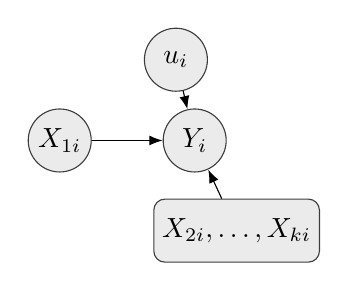
\begin{tikzpicture}[node distance=0.45cm and 0.9cm]
    \node[state] (x) at (0,0) {$X_{1i}$};
    \node[state] (y) [right =of x] {$Y_i$};
    \node[state] (u) [above right =of x] {$u_i$};
    \node[control] (c) [below right =of x] {$X_{2i},\dots,X_{ki}$};
    \path (x) edge (y);
    \path (u) edge (y);
    \path (c) edge (y);
  \end{tikzpicture}\\[0.3em]
  {\footnotesize No dashed arrows: $X_{1i}$ is unrelated to controls and $u_i$.}
  \end{column}
  \end{columns}
  \medskip
  Regression $Y_i = \beta_0 + \beta_1 X_{1i} + u_i$ gives $\hat\beta_1 = \bar Y_{X_1=1} - \bar Y_{X_1=0}$; controls are optional (precision only).\\
  \textbf{Benchmark:} each quasi-experimental design seeks a comparison where selection bias is (credibly) zero.
\end{frame}

\section{Regression as a Tool}

\begin{frame}{MLR and Conditional Mean Independence}
\linespread{1.2}\selectfont
  \[
    Y_i = \beta_0 + \beta_1 X_{1i} + \beta_2 X_{2i} + \dots + \beta_k X_{ki} + u_i
  \]
  \begin{block}{Exogeneity (MLR.4) $\leftrightarrow$ Selection on Observables}
  \[
    \E[u_i\mid X_{1i},\dots,X_{ki}]=0
    \qquad\leftrightarrow\qquad
    \big(Y_i(1),Y_i(0)\big)\indep X_{1i} \mid X_{2i},\dots,X_{ki}
  \]
  \end{block}
  ``Once we compare units with the same controls, treatment is as good as random.''
  \medskip

  \begin{itemize}
    \item $\hat\beta_j$ \emph{always} estimates a partial correlation.
    \item It is a causal effect \emph{only if} this assumption holds, and the assumption can never be tested directly: we cannot check that no relevant variable is missing.
  \end{itemize}
\end{frame}

\begin{frame}{Controls Can Change Everything: School Budget Example}
\linespread{1.2}\selectfont
  \centering
  \begin{tabular}{lcc}
    \toprule
    & \multicolumn{2}{c}{Dependent variable: \texttt{math4}} \\
    & (1) & (2) \\
    \midrule
    Expenditure per student (\$1000) & $-0.570$ & $2.083^{***}$ \\
    & $(0.428)$ & $(0.350)$ \\
    Share eligible for free lunch & & $-0.471^{***}$ \\
    & & $(0.014)$ \\
    \midrule
    Observations & 1,823 & 1,823 \\
    $R^2$ & 0.001 & 0.368 \\
    \bottomrule
  \end{tabular}
  \medskip

  \raggedright
  Adding one control flips the sign. Is column (2) causal? Only if nothing else in $u_i$ correlates with spending, \emph{conditional on lunch}. Can we be sure?
\end{frame}

\begin{frame}{What Variation Identifies $\hat\beta_1$? Frisch--Waugh}
\linespread{1.2}\selectfont
  \[
    Y_i = \beta_0 + \beta_1 X_{1i} + \bm{X}_{2i}'\bm\beta_2 + u_i
  \]
  \begin{enumerate}
    \item Regress $X_{1i}$ on $\bm X_{2i}$, keep residuals $\tilde X_{1i}$
    \item Regress $Y_i$ on $\bm X_{2i}$, keep residuals $\tilde Y_i$
    \item Regress $\tilde Y_i$ on $\tilde X_{1i}$ $\Rightarrow$ slope $=\hat\beta_1$ from the full MLR
  \end{enumerate}
  \medskip
  \begin{itemize}
    \item $\hat\beta_1$ uses only the variation in $X_1$ that the controls do \emph{not} explain.
    \item \textbf{Bridge:} panel fixed effects are Frisch--Waugh with unit dummies as $\bm X_2$. Partialling out the dummies is the same as demeaning each unit's data (the ``within'' transformation).
  \end{itemize}
\end{frame}

\begin{frame}{Interpreting Coefficients: The Building Blocks}
\linespread{1.2}\selectfont
  \textbf{Dummies and interactions}
  \[
    Y_i = \beta_0 + \beta_1 D_i + \beta_2 X_i + \beta_3 (D_i\times X_i) + u_i
  \]
  Slope of $X$: $\beta_2$ if $D_i=0$; $\beta_2+\beta_3$ if $D_i=1$. Jump at $X_i=0$: $\beta_1$.
  \medskip

  \begin{columns}[T]
    \begin{column}{0.48\textwidth}
      \textbf{Logs}\\[2pt]
      \begin{tabular}{@{}ll@{}}
        \toprule
        Model & Interpretation of $\beta$ \\
        \midrule
        level--level & $\Delta Y=\beta\,\Delta X$ \\
        level--log & $\Delta Y=(\beta/100)\,\%\Delta X$ \\
        log--level & $\%\Delta Y\approx(100\beta)\,\Delta X$ \\
        log--log & $\%\Delta Y=\beta\,\%\Delta X$ \\
        \bottomrule
      \end{tabular}
    \end{column}
    \begin{column}{0.48\textwidth}
      \textbf{Where they reappear}\\[2pt]
      \begin{itemize}
        \item DiD: $\text{Treat}_i\times\text{Post}_t$
        \item Panel FE: one dummy per unit
        \item RDD: cutoff dummy $\times$ running variable
        \item Event study: one dummy per period relative to treatment
        \item Log outcomes $\Rightarrow$ effects in \%
      \end{itemize}
    \end{column}
  \end{columns}
\end{frame}

\section{Why OLS Fails}

\begin{frame}{The Master Formula}
\linespread{1.2}\selectfont
  Simple regression $Y_i=\beta_0+\beta_1X_i+u_i$. Under MLR.1--MLR.3:
  \begin{block}{Probability Limit of OLS}
  \[
    \hat\beta_1 \xrightarrow{p} \beta_1 + \frac{\Cov(X_i,u_i)}{\Var(X_i)}
  \]
  \end{block}
  \begin{itemize}
    \item Exogeneity $\Rightarrow\Cov(X_i,u_i)=0\Rightarrow$ OLS is consistent for the causal $\beta_1$.
    \item Endogeneity $\Rightarrow$ OLS is inconsistent: more data does \emph{not} help.
    \item The sign of $\Cov(X_i,u_i)$ gives the direction of the bias.
  \end{itemize}
  \medskip
  Three common reasons why $\Cov(X_i,u_i)\neq 0$:
  \textbf{omitted variables}, \textbf{measurement error}, \textbf{reverse causality}.
\end{frame}

\begin{frame}{Omitted Variable Bias}
\linespread{1.2}\selectfont
  True model: $\log(wage_i) = \beta_0 + \beta_1 educ_i + \beta_2 ability_i + u_i$\\
  Estimated:  $\log(wage_i) = \beta_0 + \beta_1 educ_i + v_i$, \quad $v_i=\beta_2\,ability_i+u_i$
  \[
    \hat\beta_1 \xrightarrow{p} \beta_1 + \beta_2\cdot\frac{\Cov(educ_i,ability_i)}{\Var(educ_i)}
  \]
  \centering
  \begin{tabular}{lcc}
    \toprule
    & $\Cov(X_1,X_2)>0$ & $\Cov(X_1,X_2)<0$ \\
    \midrule
    $\beta_2>0$ & upward bias & downward bias \\
    $\beta_2<0$ & downward bias & upward bias \\
    \bottomrule
  \end{tabular}
  \medskip

  \raggedright
  Ability raises wages and correlates with schooling $\Rightarrow$ OLS overstates the return to education.\\
  \textbf{Bridge:} if the omitted variable is fixed over time (ability), panel FE and DiD remove it.
\end{frame}

\begin{frame}{Measurement Error and Reverse Causality}
\linespread{1.2}\selectfont
  \textbf{Classical measurement error in $X$:} observe $\widetilde{educ}_i = educ_i + w_i$, with $w_i$ pure noise.
  \[
    \hat\beta_1 \xrightarrow{p} \beta_1\cdot\underbrace{\frac{\Var(educ_i)}{\Var(educ_i)+\Var(w_i)}}_{\in(0,1]}
    \qquad\Rightarrow\text{ attenuation bias towards zero}
  \]
  \textbf{Reverse causality (simultaneity):}
  \begin{align*}
    grades_i  &= \beta_0 + \beta_1\,funding_i + u_i\\
    funding_i &= \delta_0 + \delta_1\,grades_i + v_i
  \end{align*}
  $funding_i$ depends on $grades_i$, which depends on $u_i$ $\Rightarrow \Cov(funding_i,u_i)\neq0$, even if $\Cov(u_i,v_i)=0$.
  \medskip

  \textbf{Bridge:} adding controls fixes neither problem. Both are classic motivations for IV.
\end{frame}

\begin{frame}{The Limits of ``Just Add Controls''}
\linespread{1.2}\selectfont
  \begin{itemize}
    \item Adding every relevant covariate would remove the bias, but we can never verify that we have them all.
    \item Some confounders are unobservable by nature (ability, motivation, local politics).
    \item Controls do not solve measurement error or reverse causality.
    \item ``Bad controls'': controlling for a variable that is itself an outcome of treatment introduces bias.
  \end{itemize}
  \medskip
  \textbf{Modern approach:} instead of trying to observe every confounder, find a \emph{source of variation} in $X$ that is plausibly unrelated to the confounders.
  \medskip

  That source of variation is the \emph{research design}.
\end{frame}

\section{Inference}

\begin{frame}{Sampling Distribution of $\hat\beta$}
\linespread{1.2}\selectfont
  The \textbf{estimator} $\hat\beta$ is a random variable: each sample gives a different \textbf{estimate}.
  \medskip

  \begin{itemize}
    \item \textbf{Unbiased:} $\E[\hat\beta]=\beta$ (holds in any sample size)
    \item \textbf{Consistent:} $\hat\beta\xrightarrow{p}\beta$ as $n\to\infty$
    \item \textbf{Asymptotically normal:} $\hat\beta \overset{a}{\sim} N\!\left(\beta,\ \Var(\hat\beta\mid\bm X)\right)$
  \end{itemize}
  \medskip
  OLS under MLR.1--MLR.4 has all three.\\
  \textbf{Bridge:} the IV estimator is consistent but \emph{biased} in finite samples (towards OLS), and the bias is severe when the instrument is weak.
\end{frame}

\begin{frame}{The Sandwich and Robust Standard Errors}
\linespread{1.2}\selectfont
  \[
    \Var(\hat{\bm\beta}\mid\bm X) = (\bm X'\bm X)^{-1}\;\bm X'\,\E[\bm u\bm u'\mid\bm X]\,\bm X\;(\bm X'\bm X)^{-1}
  \]
  Everything depends on the middle term, $\bm\Omega=\E[\bm u\bm u'\mid\bm X]$:
  \medskip

  \begin{tabular}{@{}lll@{}}
    \toprule
    Assumption on $\bm\Omega$ & Estimator & Status \\
    \midrule
    $\sigma^2_u\bm I_n$ (homoskedastic) & default \texttt{lm()} SEs & rarely credible \\
    $\mathrm{diag}(\sigma^2_1,\dots,\sigma^2_n)$ & HC robust: $\hat\sigma^2_i=\hat u_i^2$ & cross-section default \\
    block-diagonal by cluster & cluster-robust & panel / DiD default \\
    \bottomrule
  \end{tabular}
  \medskip

  Variance drivers (homoskedastic case):
  $\Var(\hat\beta_j\mid\bm X)=\dfrac{1}{n}\cdot\dfrac{\sigma_u^2}{\sigma^2_{X_j}}\cdot\dfrac{1}{1-R_j^2}$\\
  \textbf{Bridge:} FE and IV use less variation in $X_j$, so their standard errors are larger.
\end{frame}

\begin{frame}{Clustered Standard Errors: Why}
\linespread{1.2}\selectfont
  MLR.3 (random sampling) implies $\E[u_iu_j\mid\bm X]=0$ for $i\neq j$. This fails when observations share shocks:
  \begin{itemize}
    \item Students in the same school; firms in the same region
    \item The same unit observed over time (panel): serially correlated $u_{it}$
    \item Treatment assigned at group level (a policy in some states)
  \end{itemize}
  \medskip
  \textbf{Moulton factor} (equal-sized groups of size $\bar n$):
  \[
    \frac{\Var_{\text{true}}(\hat\beta)}{\Var_{\text{iid}}(\hat\beta)} \approx 1 + (\bar n-1)\,\rho_X\,\rho_u
  \]
  $\rho_X,\rho_u$: within-cluster correlation of regressor and error. If $X$ is constant within clusters ($\rho_X=1$) and groups are large, iid SEs can be wildly too small.
\end{frame}

\begin{frame}[fragile]{Clustered Standard Errors: How}
\linespread{1.2}\selectfont
  Allow arbitrary correlation \emph{within} clusters $g=1,\dots,G$, independence \emph{across} them:
  \[
    \widehat{\Var}_{CL}(\hat{\bm\beta})=(\bm X'\bm X)^{-1}\Big(\sum_{g=1}^{G}\bm X_g'\,\hat{\bm u}_g\hat{\bm u}_g'\,\bm X_g\Big)(\bm X'\bm X)^{-1}
  \]
  (in practice multiplied by a small-sample correction $\frac{G}{G-1}\frac{n-1}{n-k-1}$)
  \medskip

  \textbf{Practical rules}
  \begin{itemize}
    \item Cluster at the level at which treatment is assigned (Abadie et al., 2023).
    \item Panel/DiD: cluster by unit to allow serial correlation (Bertrand, Duflo \& Mullainathan, 2004).
    \item Asymptotics are in $G$, not $n$: with few clusters ($G\lesssim 30$--$50$) use the wild cluster bootstrap.
  \end{itemize}
  \begin{lstlisting}
library(fixest)
feols(y ~ x | unit + year, data = df, cluster = ~unit)
  \end{lstlisting}
\end{frame}

\begin{frame}{Tests and Confidence Intervals: Correct Interpretation}
\linespread{1.2}\selectfont
  $t$-statistic: $T=\dfrac{\hat\beta_j-\beta_{j,0}}{\SEhat(\hat\beta_j)}\overset{a}{\sim}N(0,1)$ under $H_0$. Reject at level $\alpha$ if $|T|>z_{1-\alpha/2}$.
  \medskip

  \begin{itemize}
    \item \textbf{p-value:} the probability, \emph{if $H_0$ were true}, of a test statistic at least as extreme as the one observed.\\ It is \textbf{not} the probability that $H_0$ is true.
    \item \textbf{95\% CI} $[\hat\beta_j\pm1.96\,\SEhat(\hat\beta_j)]$: across repeated samples, 95\% of intervals constructed this way cover $\beta_j$. A given realized interval either contains $\beta_j$ or it does not.
    \item \textbf{Statistical vs.\ economic significance:} report effect sizes (e.g.\ the effect of a 1-SD change in $X_j$), not just stars.
  \end{itemize}
  \medskip
  The SEs (robust or clustered) determine everything on this slide, so choosing them is a substantive decision.
\end{frame}

\section{Bridge to Research Designs}

\begin{frame}{One Map: What Each Design Assumes Instead}
\linespread{1.2}\selectfont
  \begin{tabular}{@{}llll@{}}
    \toprule
    Design & Replaces $\E[u_i\mid X_i]=0$ with & Estimand & Inference \\
    \midrule
    RCT & Random assignment & ATE & robust \\
    MLR & Selection on observables & ATE (if CIA) & robust \\
    IV & Instrument exogenous + relevant & LATE & robust / clustered \\
    Panel FE & Strict exogeneity given unit FE & within-unit effect & cluster by unit \\
    DiD & Parallel trends & ATT & cluster by unit/group \\
    RDD & Continuity at the cutoff & local effect at cutoff & robust / bias-corrected \\
    \bottomrule
  \end{tabular}
  \medskip

  \normalsize
  Each design is still a regression. What differs is \emph{which variation} identifies $\beta$, and \emph{why} that variation is credibly unrelated to $u_i$.
\end{frame}

\begin{frame}{Instrumental Variables}
\linespread{1.2}\selectfont
  \begin{block}{Instrument Conditions (endogenous $X_i$, instrument $Z_i$)}
  \begin{enumerate}
    \item \textbf{Relevance:} $\Cov(Z_i,X_i)\neq0$ (testable: first stage)
    \item \textbf{Exogeneity / exclusion:} $\Cov(Z_i,u_i)=0$; $Z$ affects $Y$ only through $X$ (not testable)
  \end{enumerate}
  \end{block}
  \[
    \hat\beta_1^{IV}=\frac{\widehat\Cov(Z_i,Y_i)}{\widehat\Cov(Z_i,X_i)}
    =\frac{\text{reduced form}}{\text{first stage}}
    \qquad\text{(matrix: }\hat{\bm\beta}^{IV}=(\bm Z'\bm X)^{-1}\bm Z'\bm Y\text{)}
  \]
  \begin{itemize}
    \item Compare with OLS $(\bm X'\bm X)^{-1}\bm X'\bm Y$: same structure, with $\bm Z$ supplying the exogenous variation.
    \item 2SLS: regress $X$ on $Z$ (and controls), then $Y$ on $\hat X$. Use the IV routine; SEs from a manual second stage are wrong.
    \item Weak instruments: report first-stage $F$. The rule of thumb $F>10$ is now considered too lenient for $t$-based inference (Lee et al., 2022).
  \end{itemize}
\end{frame}

\begin{frame}{IV with Heterogeneous Effects: LATE}
\linespread{1.2}\selectfont
  Binary $Z_i$ and $X_i$. Potential treatments $X_i(1),X_i(0)$ define four types:
  \medskip

  \centering
  \begin{tabular}{lcc}
    \toprule
    & $X_i(0)=0$ & $X_i(0)=1$ \\
    \midrule
    $X_i(1)=1$ & complier & always-taker \\
    $X_i(1)=0$ & defier & never-taker \\
    \bottomrule
  \end{tabular}
  \medskip

  \raggedright
  With independence, exclusion, relevance and \textbf{monotonicity} (no defiers):
  \[
    \frac{\E[Y_i\mid Z_i=1]-\E[Y_i\mid Z_i=0]}{\E[X_i\mid Z_i=1]-\E[X_i\mid Z_i=0]}
    =\E[Y_i(1)-Y_i(0)\mid\text{complier}] = \text{LATE}
  \]
  IV recovers the effect only for units whose behavior the instrument changes. Different instruments $\Rightarrow$ different complier populations $\Rightarrow$ different LATEs.
\end{frame}

\begin{frame}{Panel Data and Fixed Effects}
\linespread{1.2}\selectfont
  \[
    Y_{it}=\beta_1X_{it}+\alpha_i+\lambda_t+u_{it}
  \]
  \begin{itemize}
    \item $\alpha_i$: everything about unit $i$ that is fixed over time (ability, geography, institutions), observed or not.
    \item $\lambda_t$: common shocks in period $t$. Estimate via dummies or demeaning $\ddot Y_{it}=Y_{it}-\bar Y_i$ (Frisch--Waugh).
  \end{itemize}
  \medskip
  \textbf{What carries over from the review}
  \begin{itemize}
    \item OVB: time-invariant confounders are eliminated; time-varying ones are not.
    \item Perfect multicollinearity: effects of time-invariant regressors (e.g.\ gender) cannot be estimated.
    \item Variance: only within-unit variation is used $\Rightarrow$ larger SEs; attenuation from measurement error is often worse.
    \item Inference: $u_{it}$ is serially correlated $\Rightarrow$ cluster by unit.
  \end{itemize}
\end{frame}

\begin{frame}{Difference-in-Differences}
\linespread{1.2}\selectfont
  \[
    Y_{it}=\gamma_0+\gamma_1\text{Treat}_i+\gamma_2\text{Post}_t+\delta\,(\text{Treat}_i\times\text{Post}_t)+u_{it}
  \]
  \begin{columns}[T]
    \begin{column}{0.42\textwidth}
      \centering
      \begin{tabular}{lcc}
        \toprule
        & Pre & Post \\
        \midrule
        Treated & $\gamma_0+\gamma_1$ & $\gamma_0+\gamma_1+\gamma_2+\delta$ \\
        Control & $\gamma_0$ & $\gamma_0+\gamma_2$ \\
        \bottomrule
      \end{tabular}
    \end{column}
    \begin{column}{0.56\textwidth}
      \[
        \delta=(\bar Y_{T,post}-\bar Y_{T,pre})-(\bar Y_{C,post}-\bar Y_{C,pre})
      \]
      $\delta$: the interaction coefficient from the building-blocks slide.
    \end{column}
  \end{columns}
  \medskip

  \begin{block}{Parallel Trends}
  Absent treatment, treated and control units would have followed the same path:
  \[
    \E[Y_{it}(0)-Y_{i,t-1}(0)\mid\text{Treat}_i=1]=\E[Y_{it}(0)-Y_{i,t-1}(0)\mid\text{Treat}_i=0]
  \]
  \end{block}
  \begin{itemize}
    \item Identifies the \textbf{ATT}. Level differences between groups are allowed; differences in trends are not.
    \item Cluster at the level at which treatment is assigned.
  \end{itemize}
\end{frame}

\begin{frame}{Event Studies and Staggered Adoption}
\linespread{1.2}\selectfont
  \[
    Y_{it}=\alpha_i+\lambda_t+\sum_{k\neq-1}\delta_k\,\mathbf 1[t-E_i=k]+u_{it}
  \]
  \begin{itemize}
    \item One dummy per period relative to treatment date $E_i$; $k=-1$ is omitted (perfect multicollinearity, otherwise).
    \item Plot $\hat\delta_k$ with 95\% CIs (the coefficient plot from the inference lecture).
    \item Leads ($k<-1$) near zero: consistent with parallel pre-trends. This supports the assumption but does not prove it.
  \end{itemize}
  \medskip
  \textbf{Caveat:} when units adopt treatment at different times and effects vary over time, two-way FE compares later-treated units with already-treated ones and can even flip signs (Goodman-Bacon, 2021). Use heterogeneity-robust estimators: Callaway \& Sant'Anna (2021), Sun \& Abraham (2021), de Chaisemartin \& D'Haultf{\oe}uille (2020).
\end{frame}

\begin{frame}{Regression Discontinuity Design}
\linespread{1.2}\selectfont
  Treatment switches at a cutoff $c$ of a running variable $R_i$: $X_i=\mathbf 1[R_i\geq c]$.
  \[
    Y_i=\beta_0+\tau X_i+\beta_1(R_i-c)+\beta_2 X_i\times(R_i-c)+u_i,\qquad |R_i-c|\leq h
  \]
  \begin{itemize}
    \item $\tau$: jump in $\E[Y\mid R]$ at the cutoff. Separate slopes on each side via the interaction.
    \item \textbf{Continuity:} $\E[Y_i(0)\mid R_i=r]$ and $\E[Y_i(1)\mid R_i=r]$ are continuous at $c$. Units just above and just below are comparable.
    \item Estimand: effect \emph{at the cutoff}. External validity away from $c$ is limited.
  \end{itemize}
  \medskip
  \textbf{Practice}
  \begin{itemize}
    \item Local linear fits with data-driven bandwidth $h$ and bias-corrected robust CIs (\texttt{rdrobust}). Avoid high-order global polynomials (Gelman \& Imbens, 2019).
    \item Check for manipulation of $R$ (density test) and balance of covariates at $c$.
  \end{itemize}
\end{frame}

\begin{frame}{Recap}
\linespread{1.2}\selectfont
  \begin{itemize}
    \item Causal questions come first: potential outcomes define \emph{what} we estimate (ATE, ATT, LATE).
    \item OLS estimates partial correlations. It is causal only under $\E[u_i\mid X_i]=0$, which is unverifiable with observational data.
    \item One formula diagnoses the failure: $\plim\hat\beta_1=\beta_1+\Cov(X,u)/\Var(X)$.
    \item Inference depends on $\bm\Omega$: robust SEs for cross-sections, clustered SEs whenever errors are correlated within groups.
    \item IV, FE, DiD and RDD reuse the same tools (dummies, interactions, Frisch--Waugh, the sandwich) with a different identifying assumption. The quality of a design is the credibility of that assumption.
  \end{itemize}
\end{frame}

\begin{frame}{Recommended Literature}
\linespread{1.2}\selectfont
  \begin{itemize}
    \item Angrist \& Pischke (2015), \emph{Mastering 'Metrics}: Ch.\ 1 (RCT, selection bias), 3 (IV), 4 (RDD), 5 (DiD)
    \item Angrist \& Pischke (2009), \emph{Mostly Harmless Econometrics}: Ch.\ 8 (clustering)
    \item Cunningham (2021), \emph{Causal Inference: The Mixtape}: Ch.\ 4 (potential outcomes)
    \item Huntington-Klein (2021), \emph{The Effect}
    \item Heiß, \emph{Using R for Introductory Econometrics}: implementation
  \end{itemize}
  \medskip
  Abadie, Athey, Imbens \& Wooldridge (2023, QJE); Bertrand, Duflo \& Mullainathan (2004, QJE); Goodman-Bacon (2021, JoE); Callaway \& Sant'Anna (2021, JoE); Sun \& Abraham (2021, JoE); de Chaisemartin \& D'Haultf{\oe}uille (2020, AER); Gelman \& Imbens (2019, JBES); Lee, McCrary, Moreira \& Porter (2022, AER).
\end{frame}

\end{document}
